\section{Project Properties}\label{projectProperties}

Project Properties

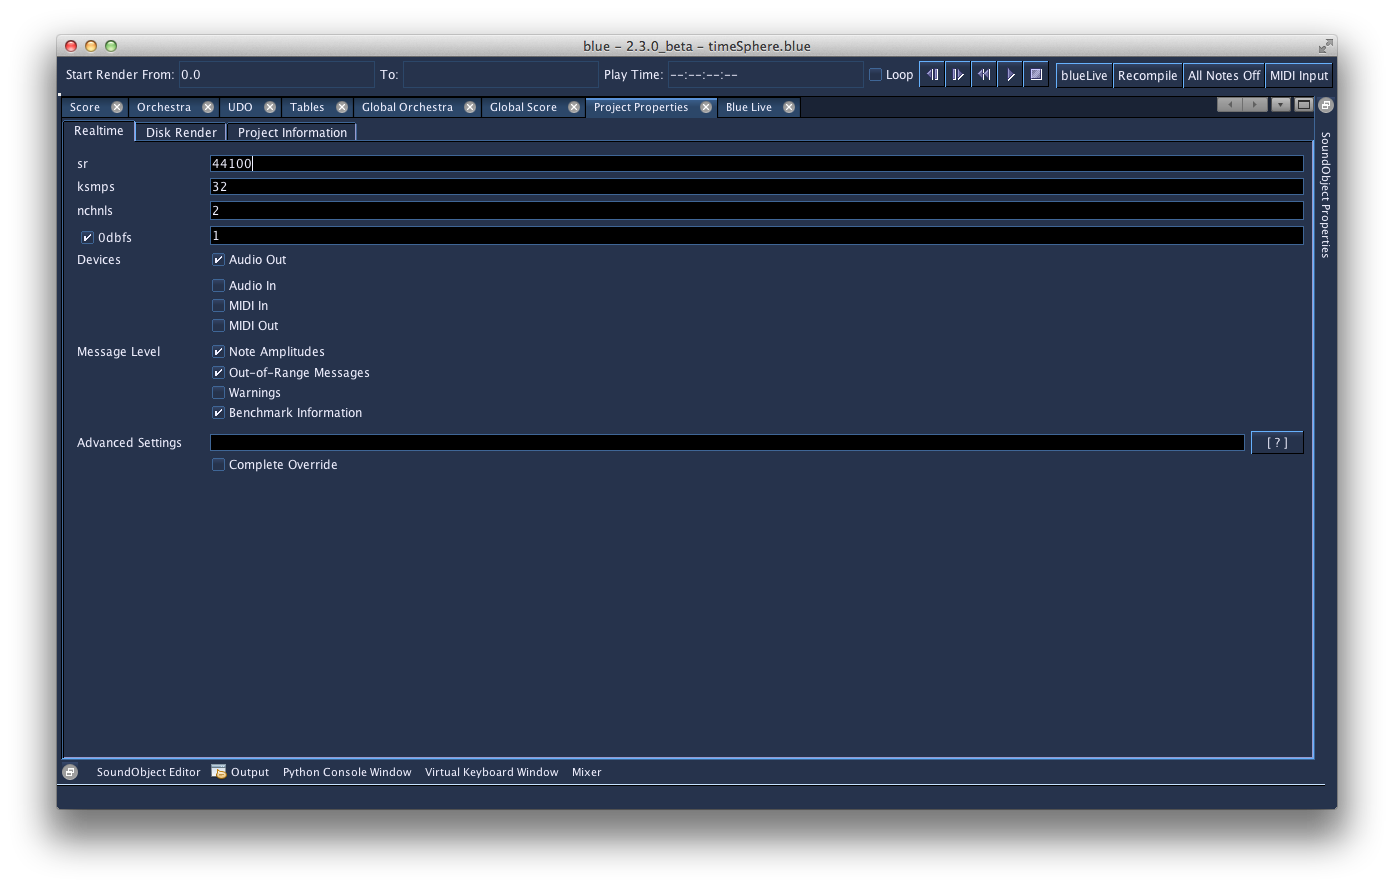
\includegraphics[width=1.00000\textwidth]{images/projectProperties.png}

\begin{description}
\item[sr]
sr to use when rendering in real-time. Value defaults to value set in
Program Options.
\item[ksmps]
ksmps to use when rendering in real-time. Value defaults to value set in
Program Options.
\item[nchnls]
nchnls to use when rendering in real-time. Value defaults to value set
in Program Options.
\item[0dbfs]
The checkbox sets whether 0dbfs is used at all in the project. If
enabled, the value will be assigned to the value in the textfield. The
default for the value is set ing Program Options, as well as if 0dbfs is
enabled by default or not.
\item[Devices]
Devices to use when rendering in real-time (Audio In/Out, MIDI In/Out).
The value of the device is dependent on the values set on the Program
Options. By delegating the value to use to what is set on the Program
Options, the project does not have to store settings which are hardware
dependent, so projects can be easily moved from one computer to the
next.

For example, if your project is set to use "Audio Out", one system may
use a value of "-+rtaudio=alsa -o dac:hw:0,0" while another system may
use a value of "-+rtaudio=winmme -o dac2". The project only needs to be
set to use "Audio Out" and when the project goes to render, the settings
set for that system's audio out will be used.
\item[Message Level]
Enables what kind of messages Csound should report. The values default
to what is set in Program Options.
\item[Advanced Settings]
Extra flags to append to the commandline that might not be covered by
options in the UI. Pressing the {[}?{]} button will open the
documentation for the Csound command flags (Csound Documentation Root
but be set for this to work).

If "Complete Override" is enabled, the value given in the "Advanced
Settings" textbox will be used as given and no other values set from the
UI will be used. Projects prior to 0.106.0 will have their commandline
settings copied to here and the "Complete Override" section will be
enabled. When this setting is enabled, the commandline should set the
call to the Csound executable to use and the flags to use but with the
name of the CSD left out as it will automatically be appended to by
blue. An example of a commandline to use here with "Complete Override"
is:

\begin{verbatim}
            csound -Wdo dac
          
\end{verbatim}
\end{description}

\begin{description}
\item[sr]
sr to use when rendering to disk. Value defaults to value set in Program
Options.
\item[ksmps]
ksmps to use when rendering to disk. Value defaults to value set in
Program Options.
\item[nchnls]
nchnls to use when rendering to disk. Value defaults to value set in
Program Options.
\item[0dbfs]
The checkbox sets whether 0dbfs is used at all in the project when
rendering to disk. If enabled, the value will be assigned to the value
in the textfield. The default for the value is set ing Program Options,
as well as if 0dbfs is enabled by default or not.
\item[Filename]
Name to use for the rendered sound file. If a value is not given, blue
will ask on each render what to name the file and where to render it to.

If the "Ask on Render" is enabled, blue will always ask on each render
what to name the file and where to render it to. This is useful to
enable if temporarily rendering parts of a project or if the project is
only meant to be used to render small sound samples.
\item[Message Level]
Enables what kind of messages Csound should report. The values default
to what is set in Program Options.
\item[Advanced Settings]
Extra flags to append to the commandline that might not be covered by
options in the UI. Pressing the {[}?{]} button will open the
documentation for the Csound command flags (Csound Documentation Root
but be set for this to work).

If "Complete Override" is enabled, the value given in the "Advanced
Settings" textbox will be used as given and no other values set from the
UI will be used. Projects prior to 0.106.0 will have their commandline
settings copied to here and the "Complete Override" section will be
enabled. When this setting is enabled, the commandline should set the
call to the Csound executable to use and the flags to use but with the
name of the CSD left out as it will automatically be appended to by
blue. An example of a commandline to use here with "Complete Override"
is:

\begin{verbatim}
            csound -Wdo mySoundFile.wav
          
\end{verbatim}
\end{description}

\begin{description}
\item[Title]
Title for this project. For general information purposes; is also used
when generating header comments in CSD.
\item[Author]
Author for this project. Defaults to value set in Program Options. For
general information purposes; is also used when generating header
comments in CSD.
\item[Notes]
Notes for this project. For general information purposes; is also used
when generating header comments in CSD.
\end{description}
